\usepackage{../pvm}

\usetikzlibrary{shadows,math}

\title{Technical Details}
\author{Fr\'ed\'eric Vogels}

\errorcontextlines 10000

\makeatletter
\pgfkeys{
  /ucll/pvm/.cd,
  start/.initial=0,
  size/.initial=1,
  height unit/.initial={0.75},
  contents/.initial={},
  id/.initial=sf,
  node style/.initial=unknown,
  stack frame/.style={minimum width=2cm,fill=red!50,font=\sc,draw},
  heap object/.style={minimum width=2cm,fill=blue!50,draw},
}
\newcommand{\alloc@block}[1][]{
  {
    \pgfkeys{
      /ucll/pvm/.cd,
      #1,
      /ucll/pvm/start/.get=\ucll@start,
      /ucll/pvm/size/.get=\ucll@size,
      /ucll/pvm/height unit/.get=\ucll@heightunit,
      /ucll/pvm/contents/.get=\ucll@contents,
      /ucll/pvm/node style/.get=\ucll@nodestyle,
      /ucll/pvm/id/.get=\ucll@id,
    }
    \tikzmath{
      real \ucll@y;
      real \ucll@height;
      \ucll@y = \ucll@start * \ucll@heightunit;
      \ucll@height = \ucll@size * \ucll@heightunit;
    }
    \node[\ucll@nodestyle,minimum height={\ucll@height cm},anchor=north west,font=\tiny] (\ucll@id) at (0,-\ucll@y) {\ucll@contents};
  }
}
\newcommand{\stackframe}[1][]{
  \alloc@block[node style=/ucll/pvm/stack frame,#1]
}
\newcommand{\heapobject}[1][]{
  \begin{scope}[xshift=2.3cm]
    \alloc@block[node style=/ucll/pvm/heap object,#1]
  \end{scope}
}

\newcommand{\memorylayout}{
  \node[anchor=south] at (1,0) {\textsc{stack}};
  \draw[fill=red!25] (-0.1,0.1) rectangle (2.1,-5.1);
  \begin{scope}[xshift=2.3cm]
    \node[anchor=south] at (1,0) {\textsc{heap}};
    \draw[fill=blue!25] (-0.1,0.1) rectangle (2.1,-5.1);
  \end{scope}
}
\makeatother

\begin{document}

\begin{frame}
  \titlepage
\end{frame}

\begin{frame}
  \frametitle{Pointers}
  \begin{itemize}
    \item Pointers have a reputation
    \item Pointers are \emph{not} hard
    \item If you can work with arrays in Java, you can work with pointers in \cpp
    \item Pointers are \emph{fragile} though
    \item Easy to make mistakes
    \item But that's ok, because they're really simple
  \end{itemize}
\end{frame}

\begin{frame}
  \frametitle{Memory: A Simple Model}
  \begin{itemize}
    \item Memory can be seen as one gigantic {\tt byte[]} array
    \item Every time you need memory (e.g.\ a stack-variable, a heap-object, \dots)
          a little part of this array is given to you
    \item You could assign ranges to the different allocation methods, e.g.
          \begin{itemize}
            \item Static allocation: first 1000000 bytes
            \item Stack: following 1000000 bytes
            \item Heap: all the rest
          \end{itemize}
          but making this distinction not important right now
  \end{itemize}
\end{frame}

\begin{frame}
  \frametitle{Memory as a {\tt byte[]}}
  \begin{center}
    \begin{tikzpicture}[scale=.25,transform shape]
      \only<2->{
        \draw[fill=red!50] (7,0) rectangle ++(4,1);
      }

      \visible<3|handout:1>{
        \foreach \i in {0,...,39} {
          \node[anchor=west,rotate=90] at ($ (\i,1) + (.5,0) $) {
            \tikzmath{
              int \address;
              \address = 4684 + \i;
               print {\tt\address};
            }
          };
        }
      }

      \visible<4-|handout:0>{
        \foreach \i in {0,...,39} {
          \node[anchor=west,rotate=90] at ($ (\i,1) + (.5,0) $) {
            \tikzmath{
              int \address;
              \address = hex(4684 + \i);
               print {\tt0x\address};
            }
          };
        }
      }
      
      \visible<0|handout:1>{
      	\foreach \i in {0,...,39} {
      		\node[anchor=west,rotate=90] at ($ (\i,2.5) + (.5,0) $) {
      			\tikzmath{
      				int \address;
      				\address = hex(4684 + \i);
      				print {\tt0x\address};
      			}
      		};
      	}
      }

      \draw (0,0) grid (40,1);
      \node[anchor=east,font=\Huge] at (0,0) {$\cdots$};
      \node[anchor=west,font=\Huge] at (40,0) {$\cdots$};
    \end{tikzpicture}
  \end{center}
  \begin{itemize}
    \item If you need an {\tt int x} variable somewhere four consecutive bytes will be required to store {\tt x}
    \item<3-> Since memory is a {\tt byte[]}, every byte has a unique index
    \item<4-> We can write this index in hexadecimal
    \item<5-> In the above figure: {\tt x} occupies bytes with indices 
              \begin{center}
                {\tt 0x1253}, {\tt 0x1254}, {\tt 0x1255}, {\tt 0x1256}
              \end{center}
    \item<5-> The index of the first byte of {\tt x} is the \emph{address} of {\tt x}
    \item<5-> Address of {\tt x} is {\tt 0x1253}
  \end{itemize}
\end{frame}

\begin{frame}
  \frametitle{A New Type}
  \begin{itemize}
    \item Say we have a variable {\tt int x}
    \item {\tt x} must have an address
    \item You can ask for this address
    \item New type: ``address of {\tt int}''
  \end{itemize}
  \vskip1cm
  \code[frame=lines,font=\small,language=c++14]{address-of.cpp}
\end{frame}

\begin{frame}
  \frametitle{What Does One Do With An Address?}
  \begin{itemize}
  \item If you know where a variable resides in memory
        (i.e.\ if you have its address), then you can read and write to it
  \end{itemize}
  \vskip1cm
  \code[frame=lines,font=\small,language=c++14]{use-address.cpp}
\end{frame}

\begin{frame}
  \frametitle{Quiz}
  \begin{itemize}
    \item Integer division {\tt x / y} has two results:
          \begin{itemize}
            \item Quotient {\tt q}
            \item Rest {\tt r}
          \end{itemize}
    \item {\tt q * y + r = x}
    \item How to write a function {\tt div} that returns quotient and rest?
  \end{itemize}
\end{frame}

\begin{frame}
  \frametitle{Div in Java: Attempt \#1}
  \code[language=java,font=\small,frame=lines]{div1.java}
  \vskip5mm
  \structure{Evaluation}
  \begin{procontralist}
    \con Need for array creation on heap (slow)
    \con Type \texttt{int[]} does not tell there will be 2 retvals
    \con Compiler does not enforce correct number of retvals
    \con Works only if function returns values of same type
    \con No naming (is {\tt q} the first or second element?)
  \end{procontralist}
\end{frame}

\begin{frame}
  \frametitle{Div in Java: Attempt \#2}
  \code[language=java,font=\small,frame=lines]{div2.java}
  \structure{Evaluation}
  \begin{procontralist}
    \pro Type safe
         \begin{itemize}
           \item \texttt{div} cannot return wrong number of results
           \item All type combinations possible
         \end{itemize}
    \pro Naming of results
    \con Need for object creation on heap (slow)
    \con Lots of ``stupid code'' necessary: we would need to define a new class for each function returning multiple values
  \end{procontralist}
\end{frame}

\begin{frame}
  \frametitle{Div in Java: Attempt \#3}
  \code[language=java,font=\small,frame=lines,width=.9\linewidth]{div3.java}
  \structure{Evaluation}
  \begin{procontralist}
    \pro Type safe
    \pro Reusable {\tt Pair} class
    \con Need for three (!) object creations on heap
    \con No naming
    \con Boilerplate code alert: {\tt Triple}, {\tt Quadruple}, \dots
  \end{procontralist}
\end{frame}

\begin{frame}
  \frametitle{Div in Java: Attempt \#4}
  \code[language=java,font=\small,frame=lines]{div4.java}
  \structure{Evaluation}
  \begin{procontralist}
    \pro Type safe
    \pro No heap allocations necessary
    \pro Clear naming
    \con Ideal, except that it doesn't work \frownie
  \end{procontralist}
\end{frame}

\begin{frame}
  \frametitle{\cpp\ To The Rescue!}
  \code[language=c++14,width=\linewidth]{div.cpp}
\end{frame}

\begin{frame}
  \frametitle{Pass-by-value vs ``Pass-by-address''}
  \begin{itemize}
    \item Passing \texttt{q} and \texttt{r} as regular \texttt{int}s does not work:
          copies are given to \texttt{div} and no matter what \texttt{div} does,
          it has no effect on \texttt{func}'s \texttt{q} and \texttt{r}
    \item Passing the \emph{addresses} of \texttt{q} and \texttt{r} allows \texttt{div} to access \texttt{func}'s local
          variables: it knows where they live!
    \item This technique is called ``out parameters'': using parameters for \emph{output}
  \end{itemize}
\end{frame}

\begin{frame}
  \frametitle{Syntax}
  \structure{Pseudosyntax}
  \code[frame=lines,language=c++14]{pointer-syntax.cpp}
  \vskip5mm
  \structure{\cpp\ syntax}
  \code[frame=lines,width=.4\linewidth,language=c++14]{pointer-syntax2.cpp}

  \begin{tikzpicture}[overlay,remember picture,box/.style={red,thick}]
    \only<2|handout:0>{
      \drawboxaround{address of int}
      \drawboxaround{int pointer}
    }
    \only<3|handout:0>{
      \drawboxaround{address of}
      \drawboxaround{address of operator}
    }
    \only<4|handout:0>{
      \drawboxaround{write to}
      \drawboxaround{write to syntax}
    }
  \end{tikzpicture}
\end{frame}

\begin{frame}
  \frametitle{Syntax}
  \begin{center}
    \begin{tabular}{ll}
      \textbf{Syntax}  & \textbf{Description} \\
      \toprule
      {\it type}*      & Pointer to a {\it type} \\
      \&{\it variable} & Address of {\it variable} \\
      *{\it pointer}   & Dereference pointer \\
    \end{tabular}
  \end{center}
  \begin{itemize}
    \item A \emph{pointer} is a variable that contains an address
    \item To access whatever is located at the address, you \emph{dereference} the pointer
    \item The {\tt \&} and {\tt *} need to be balanced
    \item Similar to arrays: given a {\tt T[] xs} you need to index {\tt xs} to reach a {\tt T}
  \end{itemize}
\end{frame}

%%% Local Variables:
%%% mode: latex
%%% TeX-master: "pointers"
%%% End:

\begin{frame}
  \frametitle{Call By Value}
  \code[frame=lines,width=.5\linewidth,font size=\small]{call-by-value.cpp}
  \begin{itemize}
    \item {\tt foo} receives a \emph{copy} of the passed object
    \item {\tt foo} knows the object's original values
    \item When {\tt foo} writes to {\tt b}, it writes to the copy
    \item {\tt foo} cannot write to the original object {\tt bar}
  \end{itemize}
\end{frame}

\begin{frame}
  \frametitle{Call By Value}
  \begin{center}
    \begin{columns}
      \column{4cm}
      \code[frame=lines,width=.95\linewidth,font size=\small]{call-by-value.cpp}
      \column{4cm}
      \begin{tikzpicture}
        \memorylayout

        \only<2->{
          \stackframe[start=0,contents={bar.x = 1}]
        }
        \only<3->{
          \stackframe[start=1,contents={bar.y = 2}]
        }
        \only<5-7>{
          \stackframe[start=2,contents={b.x = 2}]
        }
        \only<8-10>{
          \stackframe[start=2,contents={b.x = 3}]
        }
        \only<6-9>{
          \stackframe[start=3,contents={b.y = 3}]
        }
      \end{tikzpicture}
    \end{columns}
  \end{center}
  \vskip2mm
  \begin{overprint}
    \onslide<1-3>
    \begin{center}
      Creation of {\tt bar} on stack \\
      Default constructor is used
    \end{center}

    \onslide<4-6>
    \begin{center}
      Calling {\tt foo}: {\tt bar} is passed by value \\
      $\Rightarrow$ a copy is made \\
      $\Rightarrow$ copy constructor is called
    \end{center}

    \onslide<7-8>
    \begin{center}
      Incrementing {\tt b.x} operates on copy
    \end{center}

    \onslide<9-11>
    \begin{center}
      Returning from {\tt foo}: all locals are cleaned up \\
      $\Rightarrow$ {\tt b}'s destructor is called \\
    \end{center}

    \onslide<12>
    \begin{center}
      Note how {\tt bar} is still in its original state
    \end{center}
  \end{overprint}
\end{frame}


%%% Local Variables:
%%% mode: latex
%%% TeX-master: "technical-details"
%%% End:


% pass by value
% pass by pointer
% pass by reference
% return by value
% return by pointer
% return by reference
% operator = on T
% operator = on T*

\end{document}


%%% Local Variables:
%%% mode: latex
%%% TeX-master: "technical-details"
%%% End:
